\chapter{Control Strategies and State Estimation} \label{ch:controlandestimation}
rtrtrtrtr
\section{Controllability and Observability}
The controllability and observability features of the linearized system are checked using the controllability and observability Grammians $W_{c}$ and $W_{o}$ defined as
		\begin{equation}
		W_{c} = \int_{0}^{\infty}e^{At}BB^{T}e^{A^{T}t}dt,
		\end{equation}
		\begin{equation}
		W_{o} = \int_{0}^{\infty}e^{A^{T}t}C^{T}Ce^{At}dt.
		\end{equation}
As the matrices $W_{c}$ and $W_{o}$ are positive definite matrices, then the system is both controllable and observable \cite{Werner2012}.

\section{Control Strategies}
This section exposes the controllers design procedure. Here, the mathematical procedure to design a linear quadratic Gaussian controller is described. It includes a regulator and an estimator, in addition to a gain compensator, allowing the system to track a trajectory. The design process of a $H_{\infty}$ controller is shown, taking into account some weighting sensitivities.

\subsection{Linear Quadratic Regulator}
Designing an infinite-time regulator, a linear quadratic Gaussian (LQG) controller is set while looking for the minimization of the cost function $V$ as
	\begin{equation}
	V = \int_{0}^{\infty}(X^{T}QX + U^{T}RU) dt.
	\end{equation}
\\This minimization is achieved using $Q$ and $R$ as penalization matrices for the states and the inputs respectively, and the optimal input $U^{*}$ is found as
\begin{align}
\begin{split}
U^{*}&= FX,\\
F &= -R^{-1}B^{T}P,
\end{split}
\end{align}
such that $P$ is a solution of the Algebraic Riccati Equation \cite{RobustWerner2013}
	\begin{equation}
	0 = PA + A^{T}P + Q - PBR^{-1}B^{T}P.
	\end{equation}
For this quadrotor controller, the tuning matrices $Q$ and $R$ were set as $Q = C^{T}C$ and $R = 0.7* \mathcal{I}_{4\times4}$.
\\\\To find the linear quadratic estimator (LQE) gain $F_{e}$ it is used the duality principle and then, $F_{e}$ is defined as
	\begin{equation}
	F_{e} = -P_{e}C^{T}R_{e}^{-1}
	\end{equation}
	such that $P_e$ is a solution of the Filter Algebraic Riccati Equation
	\begin{equation}
	0 = P_{e}A^{T} + AP_{e} + Q_{e} - P_{e}C^{T}R_{e}^{-1}CP_{e},
	\end{equation}
setting the tuning matrices as $Q_{e} = BB^{T}$ and $R_{e} = 0.9*\mathcal{I}_{4\times4}$.
\\\\Thus, the LQG controller will be a mixture between the LQR and LQE where the closed-loop system is defined as  
\begin{align}
\label{eqn:ssgcl}
\begin{split}
\dot{X} &= (A+BF+F_{e}C)X + BU,\\
Y &= CX,
\end{split}
\end{align}
and is shown in Fig. \ref{fig:lqgsim}.
	\begin{figure}[h]
	\begin{center}
	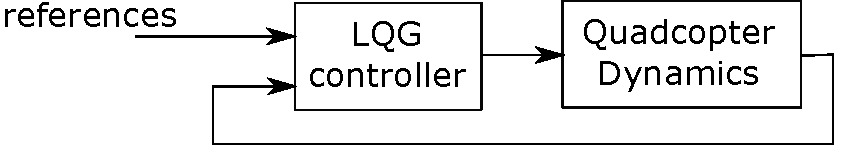
\includegraphics[width=7cm]{lqgsim.pdf}   
	\caption{Closed-loop of the controlled system with an LQG controller.}
	\label{fig:lqgsim}
	\end{center}
	\end{figure}
\\As the LQR is not made for reference tracking, to let the quadrotor track a defined trajectory, it is necessary to include a gain filter $v$ for the reference that compensates the total gain of the closed-loop system and enables the tracking of a reference input $r$. This gain filter is defined as
	\begin{equation}\label{eqn:v}
	v = -(C*(A+BF+F_{e}C)^{-1}*B)^{-1},
	\end{equation}
and its placing in the system is shown in Fig. \ref{fig:vcompensation}.
	\begin{figure}[h]
	\begin{center}
	
\includegraphics[width=4.5cm]{LQGvgain.eps}
	\caption{Closed-loop system with gain compensation for the LQG controller aiming to track a reference.}
	\label{fig:vcompensation}
	\end{center}
	\end{figure}
\\where $G_{cl}$ is the closed-system with the LQG controller described in (\ref{eqn:ssgcl}).

\subsection{$H_\infty$ Controller}
For the design of the $H\infty$ controller, a generalized plant like the shown in the Fig. \ref{fig:augmentedPlant}, was built.
\begin{figure}[h]
	\begin{center}
	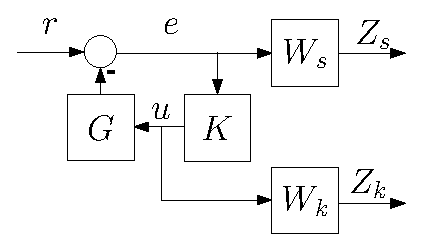
\includegraphics[width=4.5cm]{augmentedPlant.eps}
	\caption{Generalized plant with the weighting filters $W_s$ and $W_k$.}
	\label{fig:augmentedPlant}
	\end{center}
	\end{figure}	
\\\\In this generalized plant, $G$ represents the quadrotor dynamics, $K$ the controller, $r$ is the system reference, $e$ is the error, $u$ is the control input and $W_{s},\ W_{k}$ are weighting filters that must satisfy 
	\begin{equation}\label{eqn:hinf}
	\gamma = \left|\left|\begin{bmatrix}
	W_{s}S\\W_{k}KS
	\end{bmatrix}\right|\right|_{\infty} < 1,
	\end{equation}
\\where $S$ is the sensitivity function and $KS$ is the control sensitivity defined as
	\begin{equation}
	S = (\mathcal{I} + GK)^{-1},\ \ \ KS = K(\mathcal{I} + GK)^{-1}.
	\end{equation}
The weighting filters for the sensitivity and the control sensitivity were chosen as
\begin{align}\label{eqn:wswk}
\begin{split}
W_{S} &= \dfrac{w_{s}/M_{s}}{s + w_{s}}*\mathcal{I}_{4\times4}\ ,\\
W_{K} &= \dfrac{c}{M_{k}}\dfrac{s+w_{k}}{s+cw_{k}}*\mathcal{I}_{4\times4}\ ,
\end{split}
\end{align}
where $w_{s} = 10^{-4}$, $M_{s} = 10^{-4}$, $w_{k} = 20$, $M_{k} = 20$, and $c = 10^{3}$. With these weighting filters, the value of $\gamma$ is greater than one, and then it is necessary to rebuild the generalized plant using normalized weighting filters.
\\\\The $H_{\infty}$ controller can be simulated as shown in Fig. \ref{fig:hinfcontroller}.
	\begin{figure}[h]
	\begin{center}
	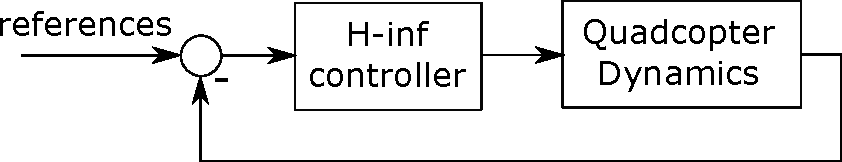
\includegraphics[width=7.0cm]{hinfcontroller.pdf}
	\caption{Closed-loop of the controlled system with an $H_{\infty}$ controller.}
	\label{fig:hinfcontroller}
	\end{center}
	\end{figure}
\subsubsection{$H_\infty$ Controller Order Reduction}
The designed $H_{\infty}$ controller for our quadrotor, will have 4 outputs (the quadrotor has 4 control inputs), 4 inputs (the quadrotor has 4 measured outputs) and 20 states (due to the 12 order plant, 4 order $W_{k}$ and 4 order $W_s$). To be able to implement this controller in a smartphone running Android, it it necessary to find a reduced order controller that behaves similarly to the full order controller $K$. To reduce the order of the controller, the singular values of the Hankel matrix
\begin{equation}
H_{k} = \begin{bmatrix}
C\\
CA\\
\vdots\\
CA^{k-1}
\end{bmatrix}
\begin{bmatrix}
B\\ AB \\ \vdots \\ A^{k-1}B
\end{bmatrix}^{T},
\end{equation}
are analysed. The energy of the Hankel singular values is shown in Fig. \ref{fig:hsv}.
\begin{figure}[h]
\begin{center}
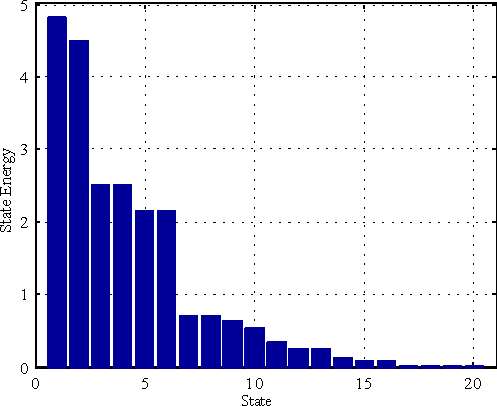
\includegraphics[width=7.8cm]{HSV.pdf}  
\caption{Hankel singular values energy histogram of the designed controller.} 
\label{fig:hsv}
\end{center}
\end{figure}
\\\\As shown in Fig. \ref{fig:hsv}, the last ordered four states have unnoticeable energy when it is plotted; that means that these four states can be truncated from the controller without modifying its dynamics \cite{Skogestad2005}. 

\section{Controllers Design}
fhfgfhfh
\subsection{Stabilize Mode}
fghgfh
\subsubsection{Dynamic Model}
rtrterere
\subsubsection{Linear Quadratic Regulator}
rtrterere

\subsubsection{$H_\infty$ Controller}
rtrtererre

\subsection{Altitude Hold Mode}
\subsubsection{Dynamic Model}
rtrterere
\subsubsection{Linear Quadratic Regulator}
rtrterere

\subsubsection{$H_\infty$ Controller}
rtrtererre

\subsection{GNSS Dependent Flight Modes}

\subsubsection{Dynamic Model}
rtrterere

\subsubsection{Linear Quadratic Regulator}
rtrterere

\subsubsection{$H_\infty$ Controller}
rtrtererre


\section{State Estimation Through Kalman Filter}
The quadrotor dynamics are sensed exclusively using the on-board smartphone's sensors. Considering that these sensors have different sample frequencies, and poor accuracy, it is necessary to use estimation algorithms, as a Kalman filter, to get reliable state data with constant sample frequency and improved accuracy and precision when compared with the raw data from the sensors.

\subsection{Attitude Estimation}
The Android API implements a Kalman filter for attitude estimation using the raw data deliverd by the smartphone's accelerometer, gyroscope and magnetometer, as exposed in \cite{Astudillo2017}. Using the quaternion $Q_s$ delivered by the Rotation virtual sensor included in the Android SDK, it is obtained an absolute orientation representation with respect to the Earth frame \cite{AndSensor}, with
\begin{align}\label{eqn:rotvector}
\begin{split}
Q_{s} &= \mathrm{e}^{(\alpha/2)(u\vv{i}+v\vv{j}+w\vv{k})} \\
&= \begin{bmatrix}
u\sin(\alpha / 2)\\
v\sin(\alpha / 2)\\
w\sin(\alpha / 2)\\
\cos(\alpha / 2)
\end{bmatrix} = \begin{bmatrix}
q_{0} \\
q_{1} \\
q_{2} \\
q_{3}
\end{bmatrix}
\end{split}
\end{align}
where $\alpha$ is the amount of degrees the quaternion is rotated around the axis $u\vv{i}+v\vv{j}+w\vv{k}$. The rotation matrix $R_{b}^{w}$ can be defined using $Q_s$ as
\begin{equation}
R_{b}^{w} = \begin{bmatrix}
1-2(q_{2}^{2}+q_{3}^{2}) & 2(q_{1}q_{2}-q_{0}q_{3}) & 2(q_{0}q_{2}+q_{1}q_{3}) \\
2(q_{1}q_{2}-q_{0}q_{3}) & 1-2(q_{1}^{2}+q_{3}^{2}) & 2(q_{2}q_{3}+q_{0}q_{1}) \\
2(q_{1}q_{3}+q_{0}q_{2}) & 2(q_{0}q_{1}+q_{2}q_{3}) & 1-2(q_{1}^{2}+q_{2}^{2})
\end{bmatrix}.
\end{equation}
Comparing the terms in the two representations of $R_{b}^{w}$, the Euler angles are obtained as
\begin{equation}\label{eqn:quattoeu}
\begin{bmatrix}
\psi \\
\theta \\
\phi
\end{bmatrix} =
\begin{bmatrix}
atan2(2(q_{3}q_{2} + q_{0}q{1}),1-2(q_{1}^{2} + q_{2}^{2})) \\
arcsin(2(q_{3}q_{1} - q_{2}q_{0})) \\
atan2(2(q_{3}q_{0} + q_{1}q{2}),1-2(q_{0}^{2} + q_{1}^{2})) 
\end{bmatrix}.
\end{equation}

\subsection{Position Estimation}
Taking into account that the global navigation satellite systems (GNSS) receivers in smartphones have an accuracy of around $3\ m$ and a sampling frequency of $1\ Hz$, a Kalman filter for position tracking is designed. In order to keep the estimation system independent from the application of controlling the quadrotor, this filter is based on the dynamics of a moving particle with constant acceleration between two samples
\begin{equation}
\xi(k+1) = \xi(k) + \dot{\xi}(k)t_{k} + 0.5\ddot{\xi}(k)t_{k}^{2},
\end{equation}
where $t_{k}$ is the sample time.\\\\
Using $E_{k} = \begin{bmatrix}
\xi & \dot{\xi} & \ddot{\xi}
\end{bmatrix}^{T}
 =
\begin{bmatrix}x_{k} & y_{k} & z_{k} & \dot{x}_{k} & \dot{y}_{k} & \dot{z}_{k} & \ddot{x}_{k} & \ddot{y}_{k} & \ddot{z}_{k} \end{bmatrix}^{T}$ as state vector and being 
\begin{equation}\label{eqn:A}
\Gamma = \begin{bmatrix}
   				 1 & 0 & 0 & t_{k} & 0 & 0 & 0.5t_{k}^{2} & 0 & 0\\
   				 0 & 1 & 0 & 0 & t_{k} & 0 & 0 & 0.5t_{k}^{2} & 0\\
   				 0 & 0 & 1 & 0 & 0 & t_{k} & 0 & 0 & t_{k}^{2}\\
   				 0 & 0 & 0 & 1 & 0 & 0 & t_{k} & 0 & 0\\
   				 0 & 0 & 0 & 0 & 1 & 0 & 0 & t_{k} & 0 \\
   				 0 & 0 & 0 & 0 & 0 & 1 & 0 & 0 & t_{k} \\
   				 0 & 0 & 0 & 0 & 0 & 0 & 1 & 0 & 0\\
   				 0 & 0 & 0 & 0 & 0 & 0 & 0 & 1 & 0\\
   				 0 & 0 & 0 & 0 & 0 & 0 & 0 & 0 & 1 
				\end{bmatrix},
\end{equation}
the matrix that satisfies $E_{k+1} = \Gamma E_{k}$, the prediction of the state $\hat{E}_{k}^{-}$ and its covariance $P_{k}^{-}$ are obtained as
\begin{equation}\label{eqn:statePrognosis}
\hat{E}_{k}^{-} = \Gamma \hat{E}_{k-1},
\end{equation}
\begin{equation}\label{eqn:covariancePrognosis}
P_{k}^{-} = \Gamma P_{k-1} \Gamma^{T} + Q_{k},
\end{equation}
where $\hat{E}_{k-1}$ is the previous estimated state, $P_{k-1}$ the previous error covariance matrix and $Q_{k}$ the process variance. The state prediction is then corrected calculating the Kalman gain vector $K_k$ as
\begin{align}\label{eqn:correctionKalman}
\begin{split}
K_{k} &= P^{-}_{k}H^{T}(HP^{-}_{k}H^{T} + R)^{-1},
\end{split}
\end{align}
and updating the state estimation $\hat{E}_{k}$ and its covariance $P_{k}$, based on the measurements $\zeta_k$ as
\begin{align}\label{eqn:correctionKalman2}
\begin{split}
\hat{E}_{k} &= \hat{E}^{-}_{k} + K_{k}(\zeta_{k} - H\hat{E}^{-}_{k}),\\
P_{k} &= (\mathcal{I} - K_{k}H)P^{-}_{k},
\end{split}
\end{align}
where $R$ is the measurement covariance matrix, $\mathcal{I}$ is the identity matrix and $H$ is the matrix that relate $\zeta_k$ and $E_k$. $H$ is defined as
\begin{equation}\label{eqn:H}
H =\begin{bmatrix}
			1 & 0 & 0 & 0 & 0 & 0 & 0 & 0 & 0\\
			0 & 1 & 0 & 0 & 0 & 0 & 0 & 0 & 0\\
			0 & 0 & 1 & 0 & 0 & 0 & 0 & 0 & 0\\
			0 & 0 & 0 & 0 & 0 & 0 & 1 & 0 & 0\\
			0 & 0 & 0 & 0 & 0 & 0 & 0 & 1 & 0\\
			0 & 0 & 0 & 0 & 0 & 0 & 0 & 0 & 1
			\end{bmatrix},
\end{equation}
considering that $\zeta_k \in R^{6}$ contains the GNSS measurements of $x_{m}$ and $y_{m}$, the barometer measurements of $z_{m}$ (in $m$), and the measurements of $\ddot{x}_{m}$, $\ddot{y}_{m}$ and $\ddot{z}_{m}$ in the Earth frame (in $m/s^{2}$).
\\\\
The $x_{m}$ and $y_{m}$ position measurements are acquired using the GNSS receiver in the smartphone. Each sample of these coordinates are initially set in an ellipsoidal representation of decimal degrees by the receiver, and then converted to a bi-dimensional representation in meter units using the cartographic projection Magna-Sirgas.
\\
The $z_{m}$ measurements are acquired using the barometric pressure sensor which delivers the pressure value $p_k$ in hPa. This signal is converted to meters as
\begin{equation}\label{eqn:hbarom}
z_{m} = 44330\left(1-\frac{p_k}{p_{0}}^{1/5.255}\right),
\end{equation}
where $p_{0}$ is the atmospheric pressure at sea level \cite{Lauszus2015}.\\\\
The remaining measurement signals are the accelerations with respect to the Earth frame, $\ddot{\xi}_{m}$. These signals are calculated using the raw acceleration measurements from the smartphone $a_{b}$, which are represented with respect to the smartphone's body frame, and the attitude quaternion $Q_s$ as
\begin{equation}
\ddot{\xi}_{m} = \begin{bmatrix}
\ddot{x}_{m} & \ddot{y}_{m} & \ddot{z}_{m}
\end{bmatrix}^{T} =Q_{s}a_{b}Q'_{s},
\end{equation}
where $Q'_{s}$ is the quaternion conjugate of $Q_{s}$.
\\\\
The vector $\zeta_k$ is then set as
\begin{equation}
\zeta_k = \begin{bmatrix}
x_{m} & y_{m} & z_{m} & \ddot{x}_{m} & \ddot{y}_{m} & \ddot{z}_{m}
\end{bmatrix}^{T}.
\end{equation}

\subsection{Particle Model}
rtrtrtrtrt

\subsection{Quadrotor Model}
ytytyttytt

\section{Conclusions}
This chapter presented the simulation and the testing of five control techniques
for the attitude control of a quadrotor. The first technique is based
on Lyapunov theory, it proved to be very reactive, especially for the yaw
angle control. However, the stabilization in the direct neighborhood of the
equilibrium point was not rigid enough to permit hover flight. The second
one is a PID controller, it proved to be well adapted to the quadrotor when
flying near hover. It was possible using this technique to successfully perform
the first autonomous flight. The PID controller was only able to control the
quadrotor in near hover and absence of large disturbances. The third one
is an LQ controller, it displayed average stabilization results. It showed to
be less dynamic than the PID. The fourth control technique is the Backstepping,
its ability to control the orientation angles in presence of relatively
high perturbations is very interesting. The sliding-mode technique is the fifth
approach, it did not provide excellent results. The switching nature of the
controller seems to be ill adapted to the dynamics of the quadrotor. The results
of all these control approaches conducted to a combination of PID and
Backstepping into the so-called Integral Backstepping. This was proposed
as a single tool to design attitude, altitude and position controllers. The
experiment has shown that OS4 is currently able to take-off, hover, land and
avoid collisions automatically. As far as we know, OS4 is the first quadrotor
practically capable of a collision avoidance maneuver.